\documentclass[10pt,a4paper]{article}

% =========================================================================
% Packages
% =========================================================================
\usepackage[utf8]{inputenc}
\usepackage[T1]{fontenc}
\usepackage{lmodern}
\usepackage{geometry}
\usepackage{graphicx}
\graphicspath{{Gambar/}}
\usepackage{amsmath,amssymb}
\usepackage{fancyhdr}
\usepackage{titlesec}
\usepackage{booktabs}
\usepackage{tabularx}
\usepackage{array}
\usepackage{caption}
\usepackage{subcaption}
\usepackage{algorithm}
\usepackage{algpseudocode}
\usepackage{hyperref}
\usepackage{microtype}
\usepackage{url}
\usepackage{cite}
\usepackage{float}
\usepackage{placeins}

% =========================================================================
% Page Geometry & Margins (EPROTIK Standard: A4 Paper, Margins: 2.5 cm all sides)
% =========================================================================
\geometry{
 a4paper,
 top=2.5cm,
 bottom=2.5cm,
 left=2.5cm,
 right=2.5cm,
 headheight=45pt,
 headsep=12pt,
 footskip=22pt
}

% Paragraph settings: Justified, single space, compact spacing for <= 10 pages
\setlength{\parindent}{0pt}
\setlength{\parskip}{4pt}
\linespread{1.0}

% Float Spacing Adjustments
\setlength{\floatsep}{8pt plus 2pt minus 2pt}
\setlength{\textfloatsep}{10pt plus 2pt minus 2pt}
\setlength{\intextsep}{8pt plus 2pt minus 2pt}

% Hyperlink configuration
\hypersetup{
 colorlinks=true,
 linkcolor=blue,
 citecolor=blue,
 urlcolor=blue
}

% =========================================================================
% Header & Footer Settings
% =========================================================================
\pagestyle{fancy}
\fancyhf{}
\fancyhead[L]{\fontsize{9pt}{11pt}\selectfont eProceeding of TIK}
\fancyfoot[R]{\fontsize{9pt}{11pt}\selectfont\thepage}
\renewcommand{\headrulewidth}{0.4pt}
\renewcommand{\footrulewidth}{0pt}

% First page header
\fancypagestyle{firstpage}{
 \fancyhf{}
 \fancyhead[L]{%
 \begin{minipage}[c]{0.78\textwidth}
 {\fontsize{10pt}{12pt}\selectfont\textbf{eProceeding of TIK}}\\[2pt]
 {\fontsize{8.5pt}{10.5pt}\selectfont E-ISSN: 2797-1724, P-ISSN: 3031-1454}\\[1pt]
 {\fontsize{8.5pt}{10.5pt}\selectfont Vol. 7 No. 1 2027 pp. 1--10}
 \end{minipage}%
 }
 \fancyhead[R]{%
 \begin{minipage}[c]{0.20\textwidth}
 \raggedleft
 \IfFileExists{Gambar/template_eprotik_image5.png}{
\includegraphics[height=1.05cm]{template_eprotik_image5.png}}{%
 \IfFileExists{Gambar/elvira_image5.png}{
\includegraphics[height=1.05cm]{elvira_image5.png}}{}%
 }
 \end{minipage}%
 }
 \fancyfoot[R]{\fontsize{9pt}{11pt}\selectfont\thepage}
 \renewcommand{\headrulewidth}{0.5pt}
 \renewcommand{\footrulewidth}{0pt}
}

% =========================================================================
% Section Headings Formatting (EPROTIK Standard)
% Level 1: 14pt Bold
% Level 2: 12pt Bold
% Level 3: 10pt Bold
% =========================================================================
\titleformat{\section}
 {\fontsize{14pt}{17pt}\bfseries}{\thesection.}{0.5em}{}
\titlespacing*{\section}{0pt}{10pt}{3pt}

\titleformat{\subsection}
 {\fontsize{12pt}{15pt}\bfseries}{\thesubsection}{0.5em}{}
\titlespacing*{\subsection}{0pt}{7pt}{2pt}

\titleformat{\subsubsection}
 {\fontsize{10pt}{12pt}\bfseries}{\thesubsubsection}{0.5em}{}
\titlespacing*{\subsubsection}{0pt}{5pt}{2pt}

% Caption styles (9 pt / small)
\captionsetup{font={small},labelfont=bf,justification=centering}
\captionsetup[table]{position=top,skip=3pt}
\captionsetup[figure]{position=bottom,skip=4pt}

% =========================================================================
% Document Body
% =========================================================================
\begin{document}
\thispagestyle{firstpage}

% --- Article Title (20pt Bold, Left Aligned) ---
{\fontsize{19pt}{23pt}\bfseries\raggedright Penerapan Hybrid Recommendation System dengan Content-Based Filtering dan Euclidean Distance untuk Rekomendasi Warna Lipstik\par}
\vspace{6pt}

% --- Authors (11pt Regular) ---
{\fontsize{11pt}{13pt}\selectfont Dinda Fitria Indriana$^{1*}$, Muhammad Rizka$^{2}$, Rahmad Hidayat$^{3}$ \par}
\vspace{3pt}

% --- Affiliations (9pt) ---
{\fontsize{9pt}{11pt}\selectfont
$^{1,2,3}$ Jurusan Teknologi Informasi dan Komputer, Politeknik Negeri Lhokseumawe, Jl. Banda Aceh--Medan Km. 280,3 Buketrata, Lhokseumawe 24301, Indonesia \par}
\vspace{3pt}

% --- Corresponding Author (9pt) ---
{\fontsize{9pt}{11pt}\selectfont
*Penulis Korespondensi: \href{mailto:dindaindriana0911@gmail.com}{dindaindriana0911@gmail.com} \par}
\vspace{3pt}

% --- Open Access License (8pt) ---
{\fontsize{8pt}{10pt}\selectfont
This is an open access article under the \href{https://creativecommons.org/licenses/by-sa/4.0/}{CC-BY-SA} license.\par
\vspace{2pt}
\IfFileExists{Gambar/template_eprotik_image1.png}{
\includegraphics[height=0.45cm]{template_eprotik_image1.png}}{%
  \IfFileExists{Gambar/elvira_image1.png}{
\includegraphics[height=0.45cm]{elvira_image1.png}}{}%
}\par}

\vspace{4pt}
\noindent\rule{\textwidth}{0.4pt}
\vspace{2pt}

% --- Abstrak (14pt Heading, 10pt Content) ---
{\fontsize{14pt}{16pt}\bfseries Abstrak \par}
\vspace{3pt}

{\fontsize{10pt}{13pt}\selectfont
Pemilihan warna lipstik yang sesuai dengan karakteristik warna alami bibir umumnya masih dilakukan secara subjektif sehingga diperlukan suatu sistem yang mampu memberikan rekomendasi secara otomatis dan lebih objektif. Penelitian ini bertujuan untuk merancang dan membangun sistem rekomendasi warna lipstik berdasarkan citra bibir menggunakan pendekatan Deep Learning melalui model MobileNetV2 serta Hybrid Recommendation System. Penelitian menggunakan kombinasi dataset sekunder CelebA dan dataset primer dengan total 18.100 citra wajah tanpa penggunaan lipstik. Tahapan penelitian meliputi deteksi landmark wajah dengan MediaPipe Face Mesh, segmentasi area bibir, ekstraksi fitur warna menggunakan nilai rata-rata Red, Green, Blue (RGB), pembentukan label otomatis menggunakan algoritma K-Means Clustering ($K=3$) ke dalam kategori Pinkish, Brownish, dan Dark, klasifikasi tipe warna bibir menggunakan MobileNetV2 dengan transfer learning, serta pemberian rekomendasi warna lipstik menggunakan Hybrid Recommendation System yang menggabungkan Rule-Based Filtering dan Content-Based Filtering dengan metode Euclidean Distance. Hasil penelitian menunjukkan bahwa model MobileNetV2 mampu mengklasifikasikan tipe warna bibir dengan akurasi validasi sebesar 94,84\%. Selain itu, pada basis data 281 shade lipstik, sistem berhasil menghasilkan Top-3 rekomendasi dengan rata-rata tingkat kemiripan sebesar 93,62\% pada Top-1, 92,26\% pada Top-2, dan 91,41\% pada Top-3. Dengan demikian, sistem yang dikembangkan terbukti efektif memberikan rekomendasi warna lipstik yang objektif, akurat, dan personal sesuai karakteristik warna alami bibir pengguna.\par}

\vspace{4pt}
{\fontsize{10pt}{12pt}\selectfont\textbf{Kata kunci:} Deep Learning, MobileNetV2, Hybrid Recommendation System, Content-Based Filtering, Euclidean Distance, K-Means Clustering, Rekomendasi Warna Lipstik.\par}

\vspace{3pt}
\noindent\rule{\textwidth}{0.4pt}
\vspace{4pt}

% =========================================================================
% Section 1: Pendahuluan (14pt)
% =========================================================================
\section{Pendahuluan }

Perkembangan industri kosmetik di Indonesia mengalami peningkatan yang sangat pesat seiring dengan tingginya kesadaran masyarakat terhadap penampilan diri dan perawatan kecantikan. Berdasarkan survei pasar konsumen di Indonesia, produk riasan bibir seperti lipstik, \textit{lip cream}, dan \textit{lip tint} menduduki kategori produk kosmetik yang paling banyak digunakan oleh wanita, dengan persentase penggunaan mencapai 80,4\% \cite{jakpat2025}. Lipstik tidak hanya berfungsi sebagai pewarna bibir untuk meningkatkan estetika wajah, tetapi juga menjadi elemen penting dalam mengekspresikan karakter dan rasa percaya diri pemakainya.

Meskipun produk lipstik sangat populer, proses pemilihan warna (\textit{shade}) lipstik yang tepat sering kali menjadi tantangan bagi konsumen. Karakteristik warna dasar bibir setiap individu bersifat unik dan sangat bervariasi. Penelitian ilmiah oleh Vergnaud dkk. menunjukkan bahwa warna alami bibir dipengaruhi oleh berbagai faktor fisiologis yang kompleks, seperti konsentrasi melanin, aliran hemoglobin, ketebalan stratum korneum, etnis, dan usia \cite{vergnaud2024lip, vergnaud2023measurement}. Perbedaan pigmen dasar ini menyebabkan satu produk lipstik yang sama dapat menghasilkan tampilan warna akhir yang sangat berbeda ketika diaplikasikan pada bibir orang yang berbeda \cite{charton2026development}.

Sebagian besar konsumen masih memilih warna lipstik secara konvensional dan subjektif, misalnya dengan mencoba produk langsung menggunakan \textit{tester} di toko fisik atau hanya mengandalkan ulasan di media sosial. Metode ini memiliki risiko higienitas serta berpotensi menimbulkan kesalahan pemilihan warna ketika bertransaksi secara daring (\textit{online shopping}) \cite{katariya2025novel}. Konsumen sering kali membeli lipstik yang warnanya terlihat menarik pada model iklan atau katalog, namun tampak kusam (\textit{ashy}), terlalu pucat, atau terlalu mencolok saat diaplikasikan pada bibir mereka sendiri. Oleh karena itu, diperlukan sebuah sistem rekomendasi cerdas yang mampu menganalisis karakteristik visual warna alami bibir secara otomatis, objektif, dan memberikan rekomendasi produk yang presisi.

Perkembangan teknologi \textit{Computer Vision} dan \textit{Deep Learning} berbasis \textit{Convolutional Neural Network} (CNN) telah terbukti sangat efektif dalam mengenali pola dan fitur visual citra secara akurat \cite{szeliski2022computer, goodfellow2016deep, lecun2015deep}. Salah satu arsitektur CNN yang efisien adalah MobileNetV2, yang dirancang menggunakan \textit{inverted residuals} dan \textit{linear bottlenecks} sehingga memiliki beban komputasi ringan dan jumlah parameter yang relatif sedikit namun tetap mempertahankan akurasi tinggi \cite{sandler2018mobilenetv2, howard2017mobilenets}. Untuk mengelompokkan data warna bibir yang belum memiliki label standar, algoritma \textit{unsupervised learning} K-Means Clustering dapat digunakan untuk membentuk klasterisasi data berbasis kemiripan nilai warna RGB \cite{macqueen1967methods, pedregosa2011scikit}.

Dalam sistem rekomendasi produk, pendekatan tunggal seperti \textit{Rule-Based} atau \textit{Content-Based Filtering} sering kali memiliki keterbatasan. \textit{Rule-Based Filtering} efektif untuk menyaring kandidat berdasarkan batasan kategori tertentu, namun kaku dan tidak mampu mengukur derajat kemiripan gradasi warna secara kontinu \cite{ricci2015recommender}. Sebaliknya, \textit{Content-Based Filtering} berbasis metrik jarak seperti \textit{Euclidean Distance} mampu mengukur kedekatan fitur numerik secara presisi, namun membutuhkan ruang komputasi yang besar jika harus membandingkan seluruh katalog produk tanpa filter awal \cite{pratama2025sistem, aggarwal2016recommender}. Oleh karena itu, penggabungan keduanya ke dalam \textit{Hybrid Recommendation System} menjadi solusi ideal.

Penelitian ini bertujuan untuk merancang dan membangun sistem rekomendasi warna lipstik berdasarkan citra bibir dengan menerapkan arsitektur MobileNetV2 dan \textit{Hybrid Recommendation System} berbasis \textit{Content-Based Filtering} dan \textit{Euclidean Distance}. Sistem memanfaatkan deteksi landmark wajah MediaPipe Face Mesh \cite{lugaresi2019mediapipe} untuk segmentasi bibir secara otomatis, ekstraksi rata-rata warna RGB, pelabelan 3 kategori bibir (Pinkish, Brownish, dan Dark) melalui K-Means Clustering, klasifikasi MobileNetV2 dengan \textit{transfer learning}, serta penentuan Top-3 rekomendasi lipstik paling sesuai dari basis data 281 produk lipstik komersial.

% =========================================================================
% Section 2: Metode (14pt)
% =========================================================================
\section{Metode }

\subsection{Alur Kerja Sistem Rekomendasi Lipstik}
Penelitian ini dilaksanakan melalui tahapan sistematis yang mencakup pengumpulan data, prapemrosesan dan segmentasi citra bibir, klasterisasi warna menggunakan K-Means, klasifikasi berbasis MobileNetV2, serta rekomendasi hibrida berbasis jarak Euclidean. Diagram alir sistem disajikan pada Gambar \ref{fig:flowchart_system}.

\begin{figure}[htbp]
 \centering
 \IfFileExists{Gambar/skripsi_image28.png}{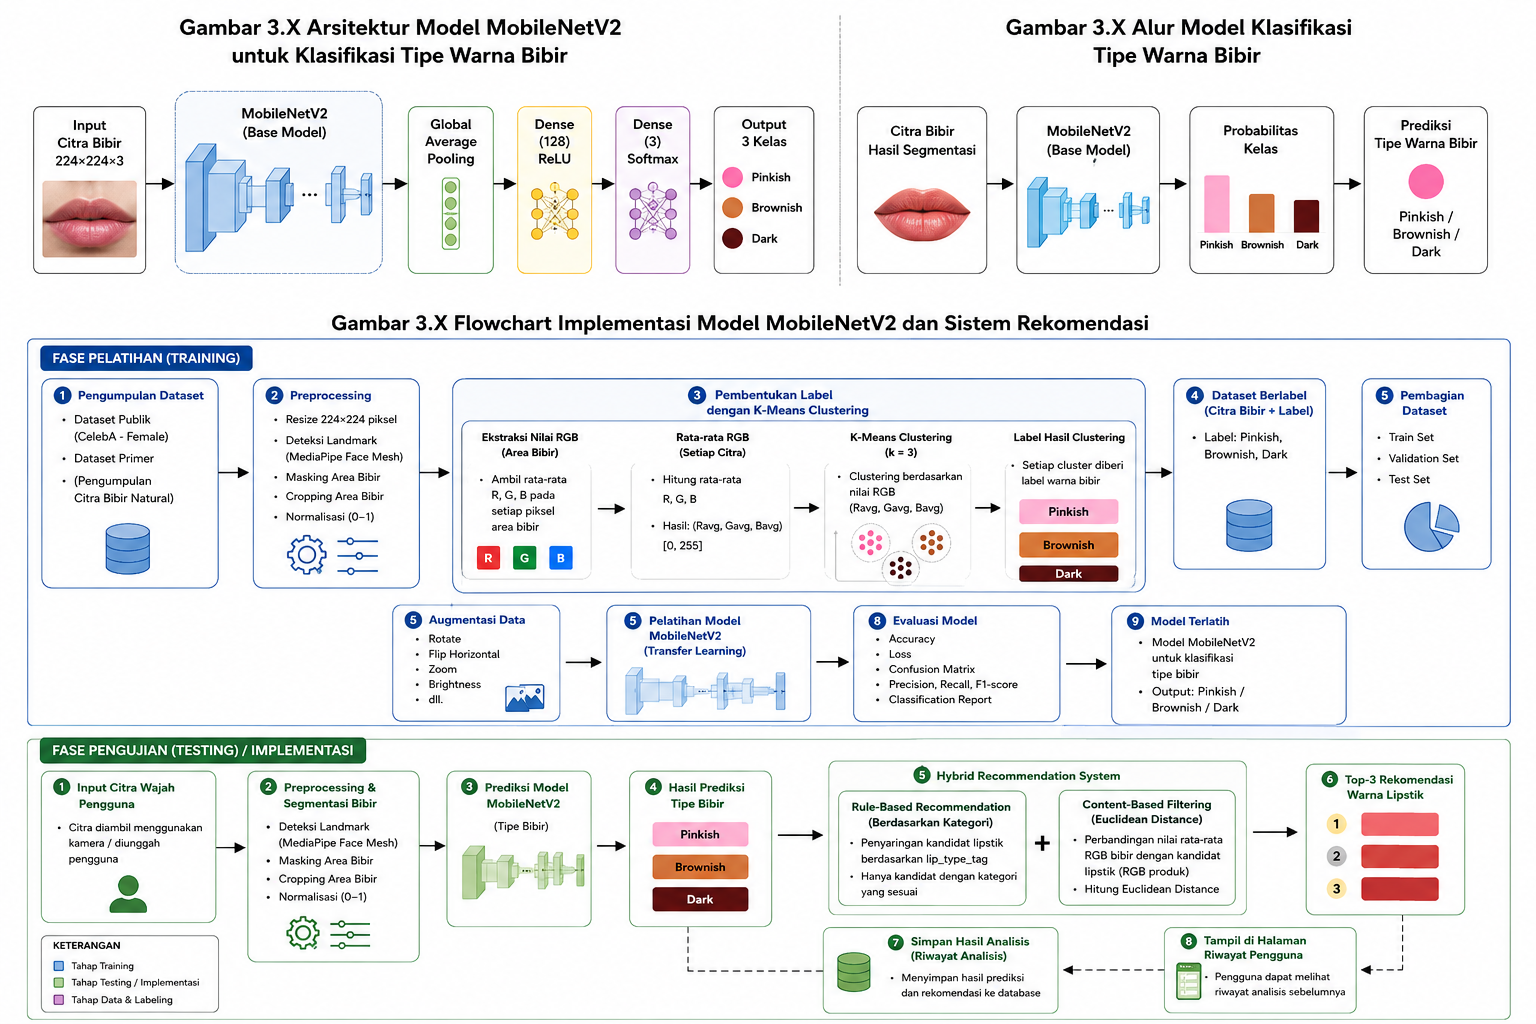
\includegraphics[width=0.62\textwidth]{skripsi_image28.png}}{\fbox{Diagram Alur Sistem}}
 \caption{Diagram Alur Sistem Rekomendasi Warna Lipstik Menggunakan MobileNetV2 dan Hybrid Recommendation System}
 \label{fig:flowchart_system}
\end{figure}

\subsection{Dataset Penelitian}
Penelitian ini menggunakan dua sumber dataset citra wajah:
\begin{enumerate}
 \item \textbf{Dataset Sekunder:} Bersumber dari \textit{Large-scale CelebFaces Attributes (CelebA) Dataset} sebanyak 18.000 citra wajah \cite{liu2015faceattributes}. Citra difilter secara ketat untuk memilih wajah tampak depan tanpa kosmetik bibir tebal.
 \item \textbf{Dataset Primer:} Pengambilan 100 citra wajah asli secara langsung menggunakan kamera beresolusi tinggi di bawah pencahayaan standar tanpa penggunaan produk riasan bibir.
\end{enumerate}
Total keseluruhan data yang digunakan adalah 18.100 citra. Dataset dibagi menjadi data latih (\textit{training set}) sebanyak 14.480 citra (80\%) dan data validasi (\textit{validation set}) sebanyak 3.620 citra (20\%).

\subsection{Prapemrosesan dan Segmentasi Bibir}
Prapemrosesan citra dilakukan melalui empat tahapan utama:
\begin{enumerate}
 \item \textbf{Deteksi Landmark Wajah:} Menggunakan pustaka Google MediaPipe Face Mesh yang memetakan 468 titik koordinat 3D pada wajah \cite{lugaresi2019mediapipe}. Sebanyak 40 titik koordinat khusus digunakan untuk mendefinisikan kontur bibir luar (\textit{outer lip}) dan bibir dalam (\textit{inner lip}) (Gambar \ref{fig:seg_bibir}(a)).
 \item \textbf{Masking Poligon:} Membentuk masker biner poligon dari indeks landmark bibir luar dan mengeliminasi area rongga mulut/gigi menggunakan landmark bibir dalam dengan fungsi \texttt{cv2.fillPoly} OpenCV \cite{bradski2000opencv}.
 \item \textbf{Ekstraksi Fitur Warna RGB Bibir:} Menghitung nilai rata-rata intensitas warna pada kanal Red ($R$), Green ($G$), dan Blue ($B$) khusus pada piksel bibir tersegmentasi (Gambar \ref{fig:seg_bibir}(b)):
 \begin{equation}
 \bar{R} = \frac{1}{N}\sum_{i=1}^{N} R_i, \quad \bar{G} = \frac{1}{N}\sum_{i=1}^{N} G_i, \quad \bar{B} = \frac{1}{N}\sum_{i=1}^{N} B_i
 \end{equation}
 di mana $N$ menyatakan total piksel aktif pada masker bibir.
 \item \textbf{Normalisasi \& Cropping ROI:} Mengonversi intensitas piksel kanal RGB ke rentang $[0, 1]$ dan memotong citra area bibir menjadi ukuran standar $224 \times 224$ piksel.
\end{enumerate}

\begin{figure}[htbp]
 \centering
 \begin{subfigure}[b]{0.48\textwidth}
 \centering
 \IfFileExists{Gambar/skripsi_image39.png}{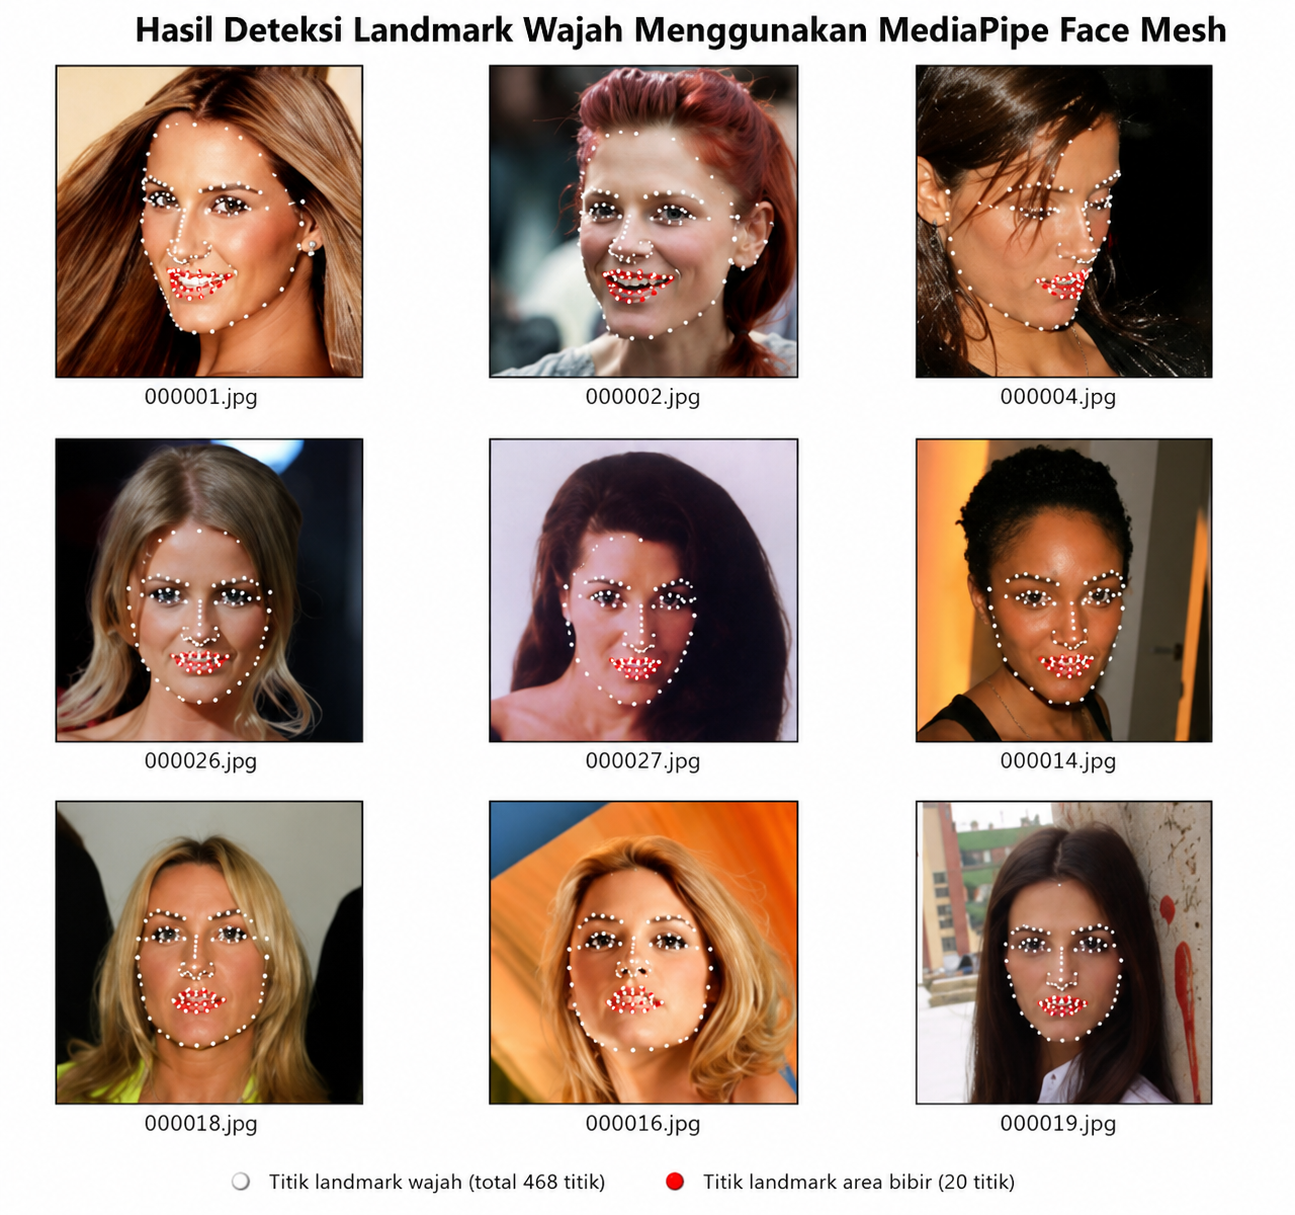
\includegraphics[width=\textwidth]{skripsi_image39.png}}{\fbox{Landmark Bibir}}
 \caption{Deteksi 40 Titik Landmark Bibir}
 \label{fig:landmark}
 \end{subfigure}
 \hfill
 \begin{subfigure}[b]{0.48\textwidth}
 \centering
 \IfFileExists{Gambar/skripsi_image40.png}{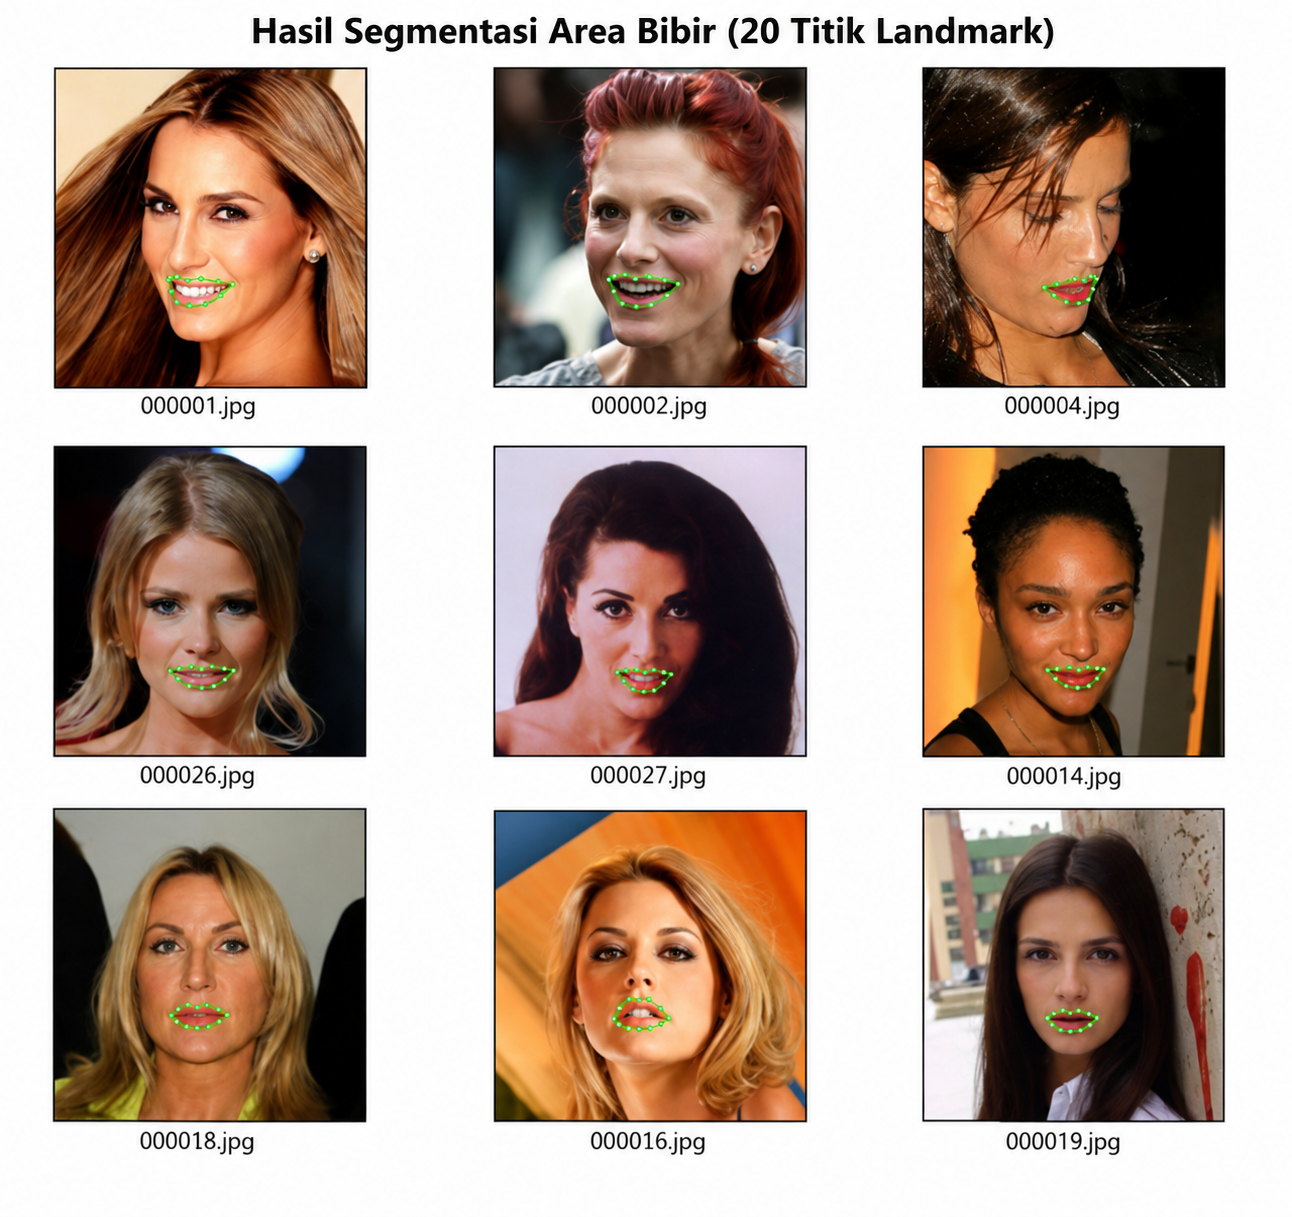
\includegraphics[width=\textwidth]{skripsi_image40.png}}{\fbox{Segmentasi Masking}}
 \caption{Hasil Segmentasi Masking Bibir}
 \label{fig:masking}
 \end{subfigure}
 \caption{Tahapan Deteksi Landmark Wajah dan Segmentasi Area Bibir Pengguna}
 \label{fig:seg_bibir}
\end{figure}

\subsection{Klasterisasi Warna Bibir dengan K-Means ($K=3$)}
Dataset citra wajah publik yang belum memiliki label diwarnai secara otomatis menggunakan algoritma K-Means Clustering berbasis vektor warna rata-rata $\mathbf{x}_i = (\bar{R}_i, \bar{G}_i, \bar{B}_i) \in \mathbb{R}^3$ \cite{macqueen1967methods}. Jumlah klaster optimal ditetapkan sebanyak $K=3$ berdasarkan hasil analisis nilai warna:
\begin{itemize}
 \item \textbf{Klaster 0 (Pinkish):} Karakteristik warna rona merah muda cerah ($\bar{R} > 160, \bar{G} > 115, \bar{B} > 110$).
 \item \textbf{Klaster 1 (Brownish):} Karakteristik warna kecokelatan/keemasan natural ($\bar{R} \approx 130\text{--}155, \bar{G} \approx 85\text{--}110, \bar{B} \approx 80\text{--}100$).
 \item \textbf{Klaster 2 (Dark):} Karakteristik warna gelap/keunguan ($\bar{R} < 125, \bar{G} < 85, \bar{B} < 80$).
\end{itemize}
Distribusi klasterisasi warna divisualisasikan pada Gambar \ref{fig:kmeans_plot}.

\begin{figure}[htbp]
 \centering
 \IfFileExists{Gambar/skripsi_image44.png}{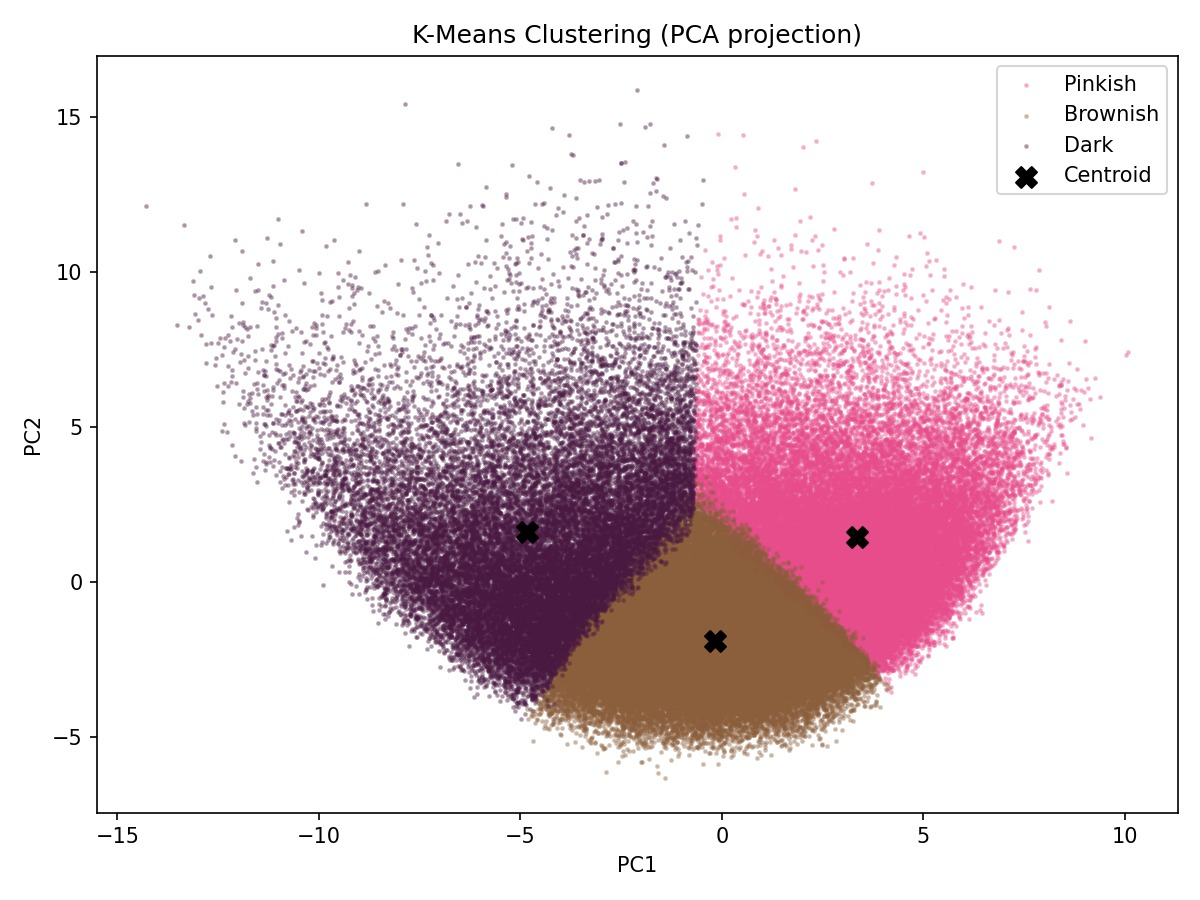
\includegraphics[width=0.64\textwidth]{skripsi_image44.png}}{\fbox{Visualisasi K-Means}}
 \caption{Visualisasi Distribusi Hasil K-Means Clustering Warna Bibir ($K = 3$)}
 \label{fig:kmeans_plot}
\end{figure}

\subsection{Arsitektur Klasifikasi MobileNetV2}
Model MobileNetV2 digunakan sebagai modul klasifikasi tipe bibir berbasis \textit{transfer learning} dengan bobot awal ImageNet \cite{sandler2018mobilenetv2}. Lapisan atas (\textit{top layer}) digantikan dengan arsitektur penyesuaian:
\begin{enumerate}
 \item \textit{Global Average Pooling 2D} untuk mereduksi dimensi spasial fitur.
 \item \textit{Dense Layer} (128 unit neuron) dengan fungsi aktivasi ReLU dan \textit{L2 Regularization} ($10^{-4}$).
 \item \textit{Dropout Layer} ($p = 0{,}4$) untuk mencegah \textit{overfitting}.
 \item \textit{Output Dense Layer} (3 unit neuron) dengan fungsi aktivasi Softmax untuk klasifikasi probabilitas multi-kelas:
 \begin{equation}
 P(y = c \mid \mathbf{x}) = \frac{e^{z_c}}{\sum_{k=1}^{3} e^{z_k}}, \quad c \in \{\text{Pinkish}, \text{Brownish}, \text{Dark}\}
 \end{equation}
\end{enumerate}
Konfigurasi hiperparameter pelatihan dirangkum pada Tabel \ref{tab:hyperparam}.

\begin{table}[htbp]
 \centering
 \caption{Parameter Hiper Pelatihan Model MobileNetV2}
 \label{tab:hyperparam}
 \fontsize{8.5pt}{11pt}\selectfont
 \begin{tabular}{ll}
 \toprule
 \textbf{Parameter Hiper} & \textbf{Nilai Konfigurasi} \\
 \midrule
 Dimensi Input Citra & $224 \times 224 \times 3$ piksel \\
 Ukuran Batch (\textit{Batch Size}) & 32 \\
 Jumlah Epoch Maksimum & 30 epoch \\
 Pengoptimal (\textit{Optimizer}) & Adam ($\beta_1 = 0{,}9, \beta_2 = 0{,}999$) \\
 Tingkat Pembelajaran (\textit{Learning Rate}) & $1 \times 10^{-4}$ (dengan \textit{ReduceLROnPlateau}) \\
 Fungsi Kerugian (\textit{Loss}) & Categorical Crossentropy \\
 Jumlah Kelas Output & 3 (Pinkish, Brownish, Dark) \\
 \bottomrule
 \end{tabular}
\end{table}

\subsection{Hybrid Recommendation System}
Setelah model MobileNetV2 memprediksi probabilitas kelas tipe bibir pengguna ($\hat{y}_{\text{user}} \in \{\text{Pinkish}, \text{Brownish}, \text{Dark}\}$), sistem merekomendasikan shade lipstik terbaik melalui mekanisme bertingkat:

\subsubsection{Tahap 1: Rule-Based Filtering}
Sistem menyaring 281 koleksi lipstik komersial pada \textit{knowledge base} berdasarkan kesesuaian atribut \texttt{lip\_type\_tag} dengan kelas prediksi pengguna:
\begin{equation}
 \mathcal{C}_{\text{kandidat}} = \{ L_j \in \mathcal{D}_{\text{lipstik}} \mid \text{tag}(L_j) = \hat{y}_{\text{user}} \}
\end{equation}
Jumlah kandidat tersaring adalah 147 produk untuk Pinkish, 127 produk untuk Brownish, dan 14 produk untuk Dark (Tabel \ref{tab:rule_based}).

\begin{table}[htbp]
 \centering
 \caption{Aturan Rule-Based Recommendation Berdasarkan Tipe Warna Bibir}
 \label{tab:rule_based}
 \fontsize{8.5pt}{11pt}\selectfont
 \begin{tabular}{cllc}
 \toprule
 \textbf{No} & \textbf{Tipe Warna Bibir Prediksi} & \textbf{Kriteria Filter Knowledge Base} & \textbf{Jumlah Kandidat Produk} \\
 \midrule
 1 & Pinkish & \texttt{lip\_type\_tag} = \textit{Pinkish} & 147 produk \\
 2 & Brownish & \texttt{lip\_type\_tag} = \textit{Brownish} & 127 produk \\
 3 & Dark & \texttt{lip\_type\_tag} = \textit{Dark} & 14 produk \\
 \midrule
 \multicolumn{3}{l}{\textbf{Total Basis Data Lipstik}} & \textbf{281 produk} \\
 \bottomrule
 \end{tabular}
\end{table}

\subsubsection{Tahap 2: Content-Based Filtering Menggunakan Euclidean Distance}
Sistem menghitung jarak geometris ruang warna RGB (\textit{Euclidean Distance}) antara vektor warna bibir pengguna $\mathbf{u} = (R_u, G_u, B_u)$ dan warna lipstik $\mathbf{v}_j = (R_j, G_j, B_j)$ pada seluruh kandidat $L_j \in \mathcal{C}_{\text{kandidat}}$:
\begin{equation}
 d(\mathbf{u}, \mathbf{v}_j) = \sqrt{(R_u - R_j)^2 + (G_u - G_j)^2 + (B_u - B_j)^2}
 \label{eq:euclidean}
\end{equation}
di mana jarak maksimum teoretis pada ruang RGB adalah $d_{\max} = \sqrt{255^2 + 255^2 + 255^2} \approx 441{,}673$.

Tingkat kemiripan warna (\textit{Similarity Score}) dihitung dalam skala persentase:
\begin{equation}
 \text{Similarity}(\mathbf{u}, \mathbf{v}_j) = \left( 1 - \frac{d(\mathbf{u}, \mathbf{v}_j)}{d_{\max}} \right) \times 100\%
 \label{eq:similarity}
\end{equation}
Sistem mengurutkan seluruh kandidat secara menaik (\textit{ascending}) berdasarkan nilai jarak $d$, kemudian memilih 3 produk teratas sebagai **Top-3 Lipstick Recommendations**. Alur algoritma rekomendasi hibrida dirangkum pada Algoritma \ref{alg:hybrid_rec}.

\begin{algorithm}[H]
\caption{Algoritma Hybrid Recommendation System untuk Rekomendasi Lipstik}
\label{alg:hybrid_rec}
\fontsize{8.5pt}{11pt}\selectfont
\begin{algorithmic}[1]
\Require Citra wajah pengguna $I_{\text{user}}$, basis data lipstik $\mathcal{D}_{\text{lipstik}}$ (281 produk), model MobileNetV2 $\mathcal{M}$
\Ensure Top-3 rekomendasi produk lipstik $\mathcal{R}_{\text{Top3}}$ beserta nilai persentase kemiripan
\State $(x_{\text{roi}}, \mathbf{u}_{\text{rgb}}) \leftarrow \text{PreprocessAndSegment}(I_{\text{user}})$ \Comment{MediaPipe Face Mesh \& Rata-rata RGB}
\State $\hat{y}_{\text{user}} \leftarrow \arg\max \mathcal{M}(x_{\text{roi}})$ \Comment{Klasifikasi tipe bibir: Pinkish / Brownish / Dark}
\State $\mathcal{C}_{\text{kandidat}} \leftarrow \emptyset$
\For{\textbf{each} produk $L_j \in \mathcal{D}_{\text{lipstik}}$}
 \If{$\text{tag}(L_j) == \hat{y}_{\text{user}}$}
 \State Hitung $d_j = \sqrt{(R_u - R_j)^2 + (G_u - G_j)^2 + (B_u - B_j)^2}$
 \State Hitung $S_j = \left(1 - \frac{d_j}{441{,}673}\right) \times 100\%$
 \State $\mathcal{C}_{\text{kandidat}} \leftarrow \mathcal{C}_{\text{kandidat}} \cup \{(L_j, d_j, S_j)\}$
 \EndIf
\EndFor
\State $\mathcal{C}_{\text{sorted}} \leftarrow \text{SortByAscendingDistance}(\mathcal{C}_{\text{kandidat}})$
\State $\mathcal{R}_{\text{Top3}} \leftarrow \text{GetTopK}(\mathcal{C}_{\text{sorted}}, K=3)$
\State \Return $\mathcal{R}_{\text{Top3}}$
\end{algorithmic}
\end{algorithm}

\subsection{Metrik Evaluasi Performa}
Evaluasi model klasifikasi MobileNetV2 diukur menggunakan metrik *Accuracy*, *Precision*, *Recall*, dan *F1-Score*:
\begin{equation}
 \text{Accuracy} = \frac{TP + TN}{TP + TN + FP + FN}
\end{equation}
\begin{equation}
 \text{Precision} = \frac{TP}{TP + FP}, \quad \text{Recall} = \frac{TP}{TP + FN}, \quad \text{F1-Score} = 2 \times \frac{\text{Precision} \times \text{Recall}}{\text{Precision} + \text{Recall}}
\end{equation}

% =========================================================================
% Section 3: Hasil dan Pembahasan (14pt)
% =========================================================================
\section{Hasil dan Pembahasan }

\subsection{Hasil Pelatihan dan Evaluasi Model MobileNetV2}
Model MobileNetV2 dilatih selama 30 epoch menggunakan dataset berlabel hasil klasterisasi K-Means. Gambar \ref{fig:eval_mobilenet}(a) menyajikan grafik konvergensi akurasi dan kerugian (\textit{loss}), sedangkan Gambar \ref{fig:eval_mobilenet}(b) menyajikan \textit{Confusion Matrix} hasil pengujian pada data validasi (803 sampel).

\begin{figure}[htbp]
 \centering
 \begin{subfigure}[b]{0.52\textwidth}
 \centering
 \IfFileExists{Gambar/skripsi_image45.png}{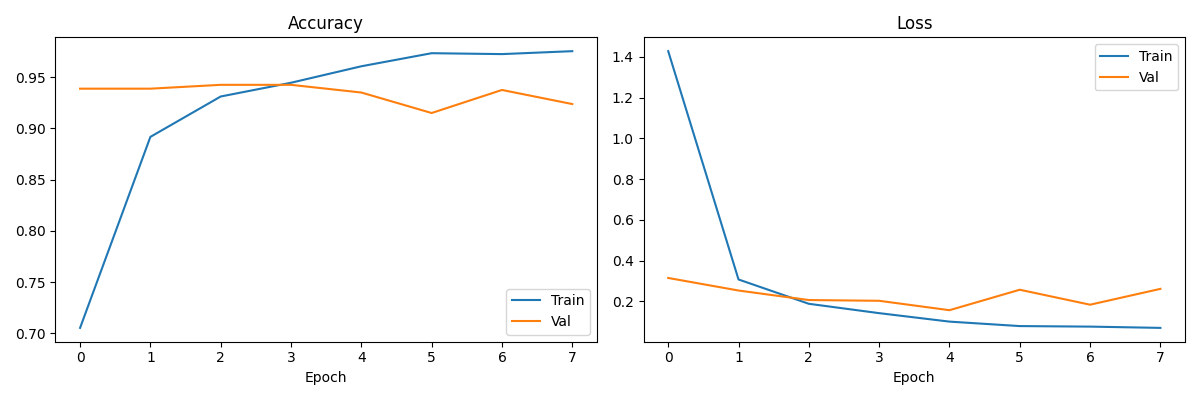
\includegraphics[width=\textwidth]{skripsi_image45.png}}{\fbox{Grafik Akurasi dan Loss}}
 \caption{Grafik Akurasi dan Loss Pelatihan}
 \label{fig:loss_acc}
 \end{subfigure}
 \hfill
 \begin{subfigure}[b]{0.44\textwidth}
 \centering
 \IfFileExists{Gambar/skripsi_image46.png}{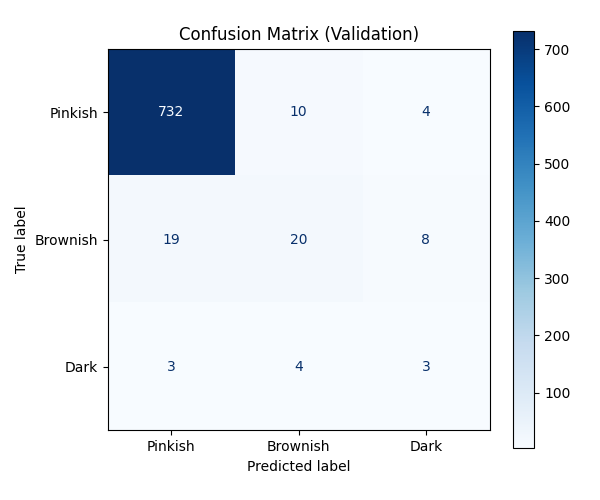
\includegraphics[width=\textwidth]{skripsi_image46.png}}{\fbox{Confusion Matrix}}
 \caption{Confusion Matrix Data Validasi}
 \label{fig:cm}
 \end{subfigure}
 \caption{Evaluasi Performa Model MobileNetV2: (a) Grafik Akurasi dan Loss, (b) Confusion Matrix pada Data Validasi}
 \label{fig:eval_mobilenet}
\end{figure}

Model mencapai konvergensi stabil pada epoch ke-15 ke atas tanpa gejala \textit{overfitting}, dengan akurasi validasi akhir sebesar \textbf{94,84\%} dan \textit{validation loss} sebesar \textbf{0,1612}. Rincian nilai metrik evaluasi per kelas dirangkum dalam \textit{Classification Report} pada Tabel \ref{tab:classification_report}.

\begin{table}[htbp]
 \centering
 \caption{Classification Report Performa Model MobileNetV2}
 \label{tab:classification_report}
 \fontsize{8.5pt}{11pt}\selectfont
 \begin{tabular}{lcccc}
 \toprule
 \textbf{Kelas Tipe Bibir} & \textbf{Precision} & \textbf{Recall} & \textbf{F1-Score} & \textbf{Support (Sampel)} \\
 \midrule
 Pinkish & 0.971 (97.1\%) & 0.981 (98.1\%) & 0.976 (97.6\%) & 746 \\
 Brownish & 0.588 (58.8\%) & 0.426 (42.6\%) & 0.494 (49.4\%) & 47 \\
 Dark & 0.200 (20.0\%) & 0.300 (30.0\%) & 0.240 (24.0\%) & 10 \\
 \midrule
 \textbf{Overall Accuracy} & \multicolumn{3}{c}{\textbf{0.940 (94.0\%)}} & \textbf{803} \\
 \textbf{Macro Average} & 0.586 & 0.569 & 0.570 & 803 \\
 \textbf{Weighted Average} & 0.939 & 0.940 & 0.938 & 803 \\
 \bottomrule
 \end{tabular}
\end{table}

Model menunjukkan performa klasifikasi sangat tinggi pada kelas \textbf{Pinkish} (F1-score 97,6\%). Pada kelas \textbf{Brownish} dan \textbf{Dark}, nilai F1-score masing-masing tercatat 49,4\% dan 24,0\%. Karakteristik ini dipengaruhi oleh dominasi citra rona cerah pada dataset publik (\textit{class imbalance}). Namun secara agregat \textit{weighted average}, model mencapai F1-score 93,8\% dan akurasi 94,0\%, membuktikan efektivitas MobileNetV2 dalam mengenali karakteristik visual bibir.

\subsection{Pengujian dan Evaluasi Hybrid Recommendation System}
Pengujian sistem rekomendasi dilakukan terhadap 30 data uji pengguna dengan variasi nilai RGB bibir yang berbeda. Sampel hasil pengujian disajikan pada Tabel \ref{tab:hasil_rekomendasi}, dan rekapitulasi performa dirangkum pada Tabel \ref{tab:rekap_similarity}.

\begin{table}[htbp]
 \centering
 \caption{Sampel Hasil Pengujian Hybrid Recommendation System pada Data Uji Pengguna}
 \label{tab:hasil_rekomendasi}
 \fontsize{8.5pt}{10.5pt}\selectfont
 \begin{tabular}{ccclccc}
 \toprule
 \textbf{No} & \textbf{RGB User} & \textbf{Tipe Bibir} & \textbf{Rekomendasi Shade} & \textbf{RGB Lipstik} & \textbf{Euclidean ($d$)} & \textbf{Similarity (\%)} \\
 \midrule
 1 & (164, 121, 108) & Pinkish & 1. Glossy Berry & (167, 97, 101) & 25.18 & 94.3\% \\
 & & & 2. Dusty Rose & (185, 115, 125) & 27.68 & 93.7\% \\
 & & & 3. Cozy Cherry & (173, 98, 94) & 28.39 & 93.6\% \\
 \midrule
 2 & (128, 102, 99) & Brownish & 1. Chilled Raspberry& (134, 85, 109) & 20.62 & 95.3\% \\
 & & & 2. Chilled Cranberry& (132, 68, 82) & 38.22 & 91.3\% \\
 & & & 3. Matte Berry & (162, 83, 86) & 41.06 & 90.7\% \\
 \midrule
 3 & (145, 98, 55) & Pinkish & 1. Satin Vermillion & (173, 95, 86) & 41.88 & 90.5\% \\
 & & & 2. Bold Ruby & (176, 88, 86) & 44.97 & 89.8\% \\
 & & & 3. Cozy Cherry & (173, 98, 94) & 48.01 & 89.1\% \\
 \midrule
 4 & (195, 167, 153) & Brownish & 1. Mauve Bliss & (170, 110, 130) & 66.36 & 85.0\% \\
 & & & 2. Warm Terracotta & (180, 105, 95) & 74.35 & 83.2\% \\
 & & & 3. Rose Brown & (160, 95, 110) & 81.12 & 81.6\% \\
 \bottomrule
 \end{tabular}
\end{table}

\begin{table}[htbp]
 \centering
 \caption{Rekapitulasi Skor Kemiripan (\textit{Similarity}) Hybrid Recommendation System}
 \label{tab:rekap_similarity}
 \fontsize{8.5pt}{11pt}\selectfont
 \begin{tabular}{lc}
 \toprule
 \textbf{Parameter Evaluasi} & \textbf{Nilai Kuantitatif} \\
 \midrule
 Jumlah Sampel Data Uji & 30 data \\
 Rata-rata Similarity Top-1 (Rekomendasi Pertama) & \textbf{93.62\%} \\
 Rata-rata Similarity Top-2 (Rekomendasi Kedua) & \textbf{92.26\%} \\
 Rata-rata Similarity Top-3 (Rekomendasi Ketiga) & \textbf{91.41\%} \\
 Nilai Similarity Tertinggi & \textbf{97.60\%} \\
 Nilai Similarity Terendah & \textbf{73.60\%} \\
 Total Basis Data Produk Lipstik Terdaftar & 281 shade \\
 \bottomrule
 \end{tabular}
\end{table}

Hasil rekapitulasi membuktikan bahwa sistem rekomendasi hibrida mampu menghasilkan rekomendasi warna lipstik dengan tingkat kecocokan yang sangat tinggi. Rata-rata kemiripan warna untuk rekomendasi utama (Top-1) mencapai \textbf{93,62\%}, dengan seluruh Top-3 rekomendasi konsisten berada di atas 91\%. Pendekatan bertingkat (\textit{two-stage hybrid}) terbukti efektif mengeliminasi ketidakcocokan kategori pada tahap \textit{Rule-Based} dan mengoptimalkan presisi gradasi warna pada tahap \textit{Euclidean Distance}.

\subsection{Implementasi Antarmuka Sistem Berbasis Web}
Sistem diimplementasikan ke dalam aplikasi web responsif. Pengguna dapat mengunggah foto wajah dan sistem secara otomatis menampilkan ROI bibir tersegmentasi, nilai RGB, kelas prediksi MobileNetV2, nilai kepercayaan (\textit{confidence}), serta kartu Top-3 rekomendasi lipstik lengkap dengan swatch warna dan skor kemiripan (Gambar \ref{fig:ui_analisis}).

\begin{figure}[htbp]
 \centering
 \IfFileExists{Gambar/skripsi_image34.png}{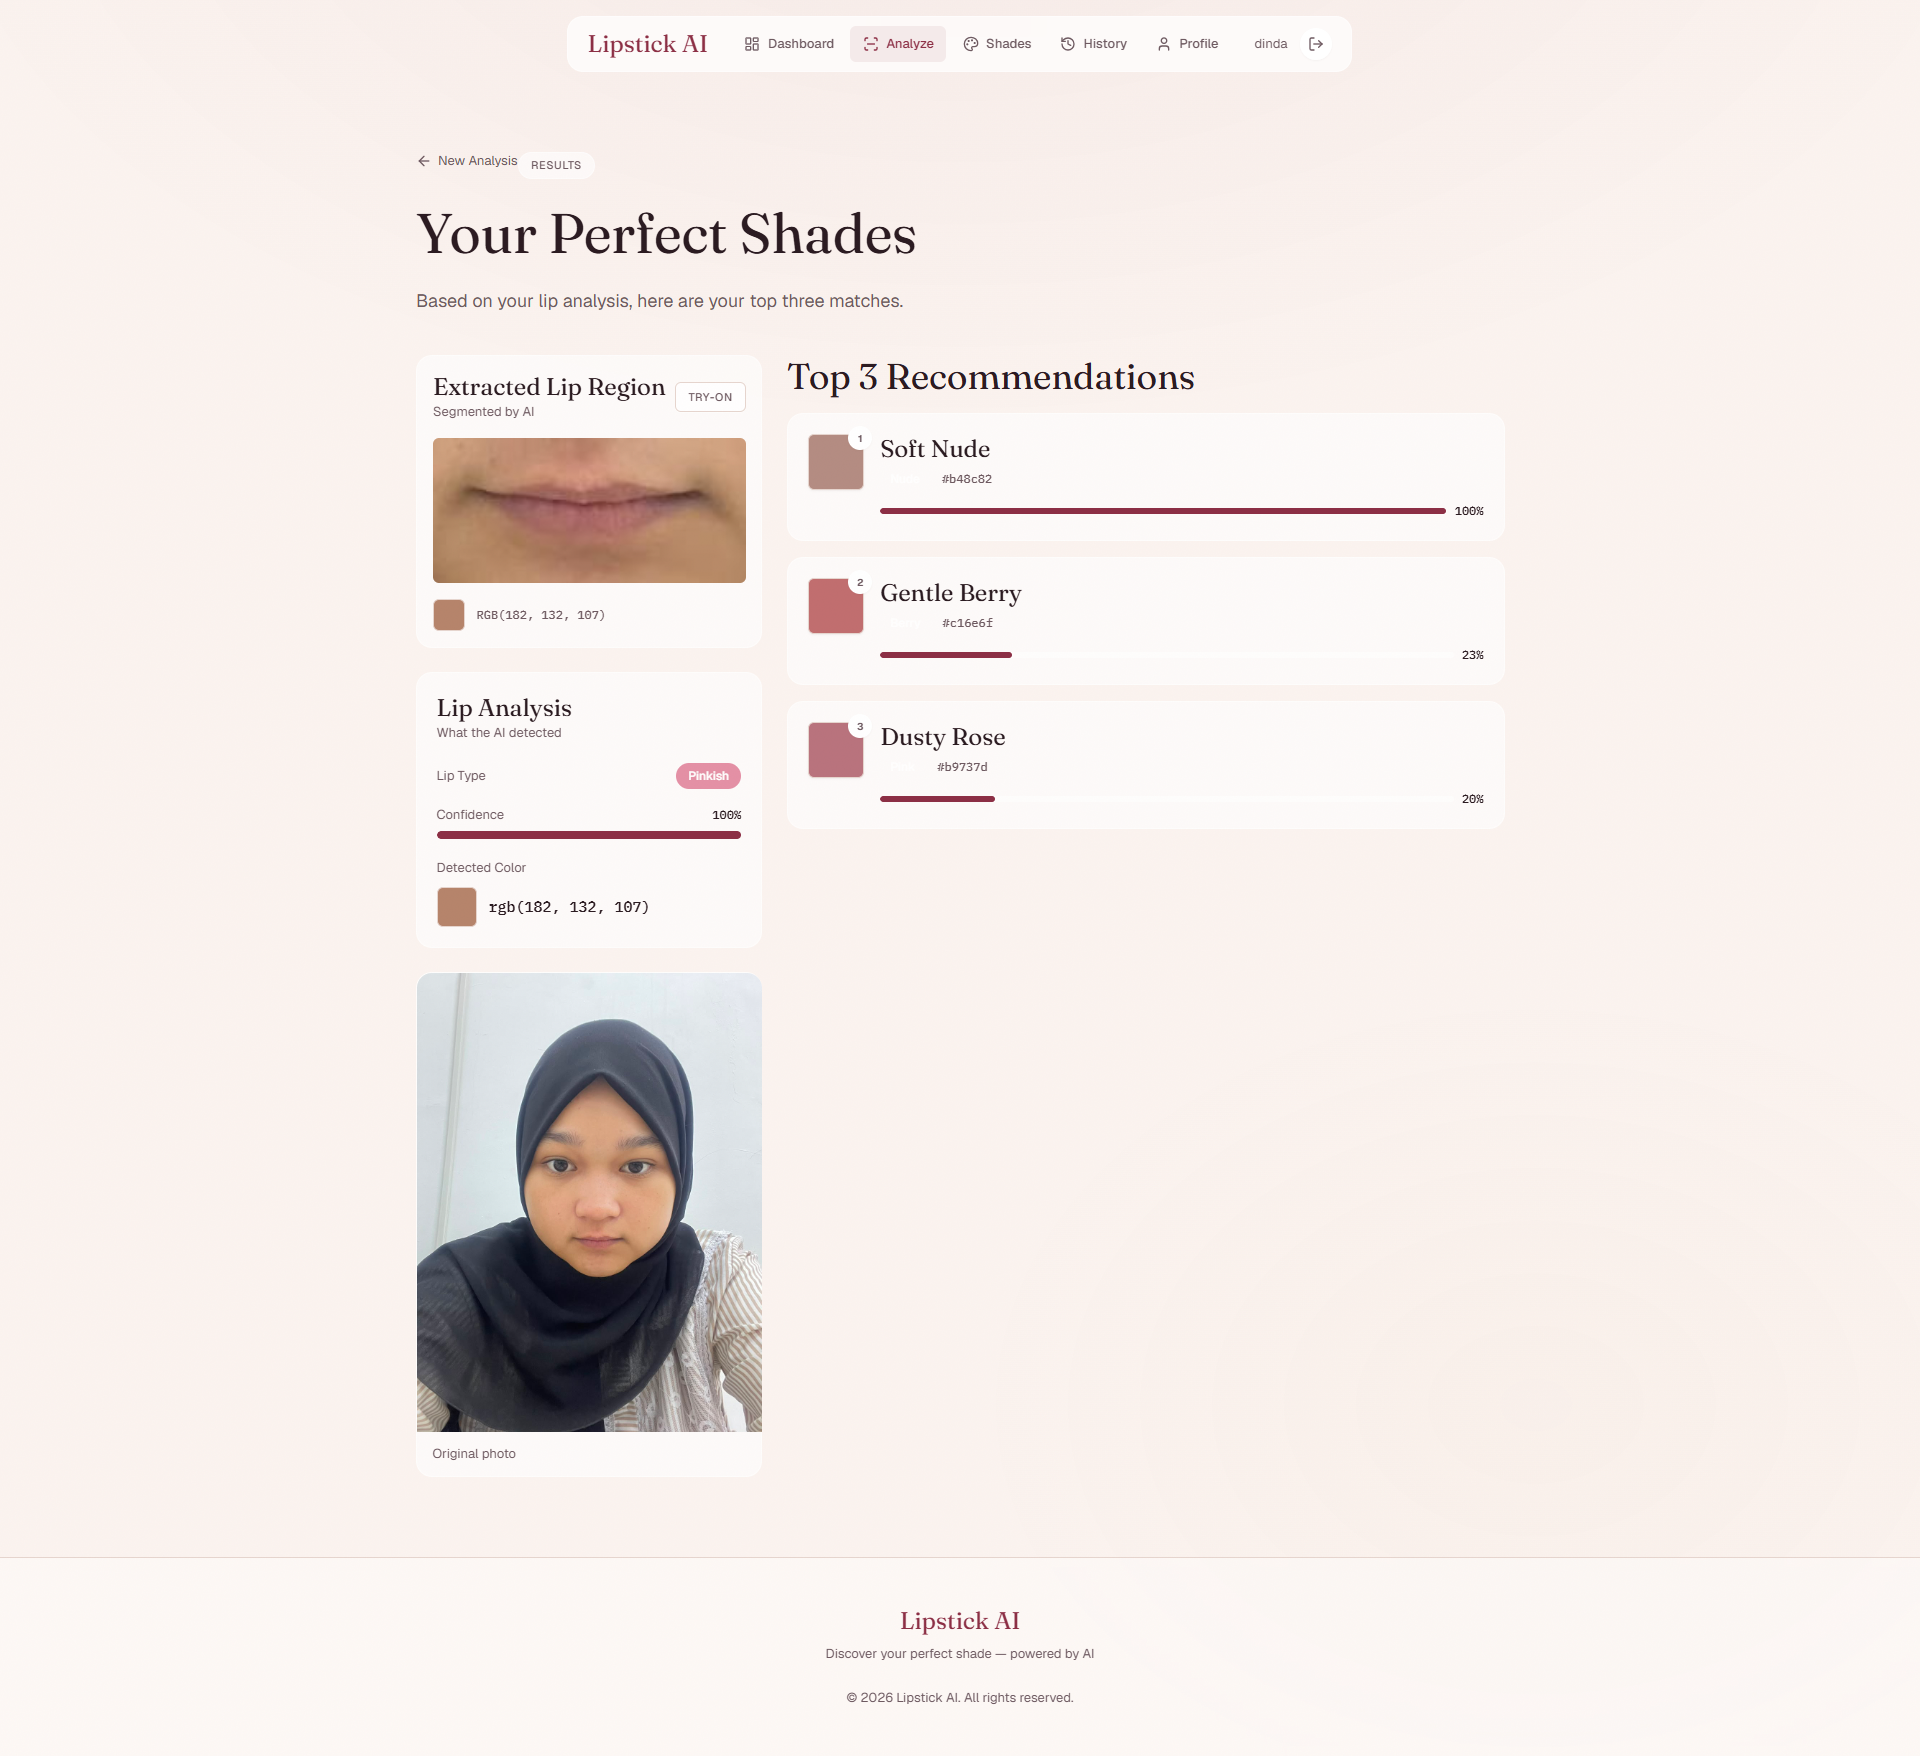
\includegraphics[width=0.55\textwidth]{skripsi_image34.png}}{\fbox{Antarmuka Hasil Analisis}}
 \caption{Implementasi Antarmuka Halaman Hasil Analisis dan Rekomendasi Lipstik}
 \label{fig:ui_analisis}
\end{figure}

\subsection{Pengujian Fungsional (Black Box Testing)}
Pengujian fungsional sistem menggunakan metode \textit{Black Box Testing} menunjukkan bahwa seluruh modul aplikasi berjalan sesuai rancangan kebutuhan fungsional dengan status \textbf{100\% PASS} (Tabel \ref{tab:blackbox}).

\begin{table}[htbp]
 \centering
 \caption{Hasil Pengujian Black Box pada Modul Analisis dan Rekomendasi}
 \label{tab:blackbox}
 \fontsize{8pt}{10pt}\selectfont
 \begin{tabularx}{\textwidth}{clXXc}
 \toprule
 \textbf{No} & \textbf{Skenario Uji} & \textbf{Aktivitas / Masukan} & \textbf{Hasil yang Diharapkan} & \textbf{Status} \\
 \midrule
 1 & Unggah Citra Valid & Foto wajah JPG/PNG & Sistem mendeteksi wajah dan menampilkan \textit{preview} & PASS \\
 2 & Deteksi Landmark & Menjalankan analisis & MediaPipe mengekstrak 468 titik landmark wajah & PASS \\
 3 & Segmentasi Bibir & Ekstraksi batas bibir & Masker poligon bibir terbentuk dan area bibir terpotong & PASS \\
 4 & Klasifikasi Warna & Ekstraksi RGB \& inferensi & MobileNetV2 memprediksi kelas (Pinkish/Brownish/Dark) & PASS \\
 5 & Rekomendasi Top-3 & Filter aturan \& jarak Euclidean & Menampilkan 3 produk lipstik dengan similarity tertinggi & PASS \\
 6 & Simpan Riwayat & Simpan ke basis data & Riwayat tersimpan dan dapat diakses pada menu \textit{History} & PASS \\
 \bottomrule
 \end{tabularx}
\end{table}

\FloatBarrier

% =========================================================================
% Section 4: Kesimpulan (14pt)
% =========================================================================
\section{Kesimpulan }

Berdasarkan hasil penelitian yang telah dilaksanakan, diperoleh kesimpulan sebagai berikut:
\begin{enumerate}
 \item Sistem rekomendasi warna lipstik berbasis citra bibir telah berhasil dibangun dengan mengintegrasikan MediaPipe Face Mesh, MobileNetV2 dengan transfer learning, dan \textit{Hybrid Recommendation System} berbasis \textit{Rule-Based Filtering} dan \textit{Content-Based Filtering} (Euclidean Distance).
 \item Model klasifikasi MobileNetV2 berhasil mengklasifikasikan tipe warna bibir pengguna ke dalam tiga kategori (Pinkish, Brownish, Dark) dengan akurasi validasi mencapai \textbf{94,84\%} dan nilai loss sebesar 0,1612.
 \item \textit{Hybrid Recommendation System} terbukti sangat efektif dalam menghasilkan rekomendasi yang personal dan objektif. Dari 281 shade lipstik, sistem menghasilkan Top-3 rekomendasi dengan rata-rata \textit{similarity} sebesar \textbf{93,62\%} pada Top-1, \textbf{92,26\%} pada Top-2, dan \textbf{91,41\%} pada Top-3, dengan tingkat kemiripan tertinggi mencapai \textbf{97,60\%}.
 \item Pengujian \textit{Black Box Testing} menunjukkan tingkat keberhasilan 100\% (PASS) untuk seluruh modul fungsional sistem.
\end{enumerate}

Saran untuk pengembangan penelitian selanjutnya antara lain:
\begin{enumerate}
 \item Menambah variasi dataset primer untuk tipe Dark dan Brownish serta menerapkan metode penyeimbangan kelas (\textit{class weight / SMOTE}) guna meningkatkan metrik performa pada kelas minoritas.
 \item Mengembangkan fitur simulasi riasan virtual (\textit{Virtual Try-On}) berbasis \textit{Augmented Reality} (AR) secara \textit{real-time}.
 \item Menambahkan parameter rona kulit (\textit{skin undertone} dan \textit{skin overtone}) serta preferensi acara untuk memperkaya faktor personalisasi rekomendasi.
\end{enumerate}

% =========================================================================
% References (IEEE Style, 12pt heading)
% =========================================================================
\section*{REFERENSI }

\begingroup
\renewcommand{\section}[2]{}%
\begin{thebibliography}{99}
\fontsize{8pt}{10pt}\selectfont
\setlength{\itemsep}{1pt}
\setlength{\parskip}{0pt}

\bibitem{jakpat2025}
Jakpat Survey, ``Makeup Product Categories Used by Indonesian Women in 2025,'' \textit{Databoks Katadata}, 2025. [Daring]. Tersedia: \url{https://databoks.katadata.co.id/en/consumer-durables-apparel/statistics/692e89e11c6f5/makeup-product-categories-used-by-indonesian-women-in-2025}.

\bibitem{vergnaud2024lip}
H. Vergnaud, Z. Charton, D. Blumenthal, V. Couturaud, M. Le Fur, E. Loescher \textit{et al.}, ``Lip Color Diversity: An Intricate Study,'' \textit{Skin Res. Technol.}, vol. 30, no. 2, p. e13583, 2024, doi: 10.1111/srt.13583.

\bibitem{vergnaud2023measurement}
H. Vergnaud, M. Cherel, G. Fran\c{c}ois, Z. Charton, E. Loescher, L. Caisey \textit{et al.}, ``Lip Color Measurement: A New Hyperspectral Imaging Device,'' \textit{Skin Res. Technol.}, vol. 29, no. 8, p. e13418, 2023, doi: 10.1111/srt.13418.

\bibitem{sandler2018mobilenetv2}
M. Sandler, A. Howard, M. Zhu, A. Zhmoginov, and L.-C. Chen, ``MobileNetV2: Inverted Residuals and Linear Bottlenecks,'' in \textit{Proc. IEEE/CVF Conf. Comput. Vis. Pattern Recognit. (CVPR)}, 2018, pp. 4510--4520, doi: 10.1109/CVPR.2018.00474.

\bibitem{gulati2023beautifai}
K. Gulati, G. Verma, M. Mohania, and A. Kundu, ``BeautifAI: Personalised Occasion-based Makeup Recommendation,'' in \textit{Proc. 14th Asian Conf. Mach. Learn. (ACML)}, PMLR, vol. 189, 2023, pp. 407--419.

\bibitem{liu2015faceattributes}
Z. Liu, P. Luo, X. Wang, and X. Tang, ``Deep Learning Face Attributes in the Wild,'' in \textit{Proc. IEEE Int. Conf. Comput. Vis. (ICCV)}, 2015, pp. 3730--3738, doi: 10.1109/ICCV.2015.425.

\bibitem{gonzalez2018digital}
R. C. Gonzalez and R. E. Woods, \textit{Digital Image Processing}, 4th ed. Harlow, England: Pearson Education Limited, 2018.

\bibitem{szeliski2022computer}
R. Szeliski, \textit{Computer Vision: Algorithms and Applications}, 2nd ed. Cham, Switzerland: Springer Nature, 2022, doi: 10.1007/978-3-030-34372-9.

\bibitem{goodfellow2016deep}
I. Goodfellow, Y. Bengio, and A. Courville, \textit{Deep Learning}. Cambridge, MA, USA: MIT Press, 2016.

\bibitem{lecun2015deep}
Y. LeCun, Y. Bengio, and G. Hinton, ``Deep Learning,'' \textit{Nature}, vol. 521, no. 7553, pp. 436--444, 2015, doi: 10.1038/nature14539.

\bibitem{pan2010survey}
S. J. Pan and Q. Yang, ``A Survey on Transfer Learning,'' \textit{IEEE Trans. Knowl. Data Eng.}, vol. 22, no. 10, pp. 1345--1359, 2010, doi: 10.1109/TKDE.2009.191.

\bibitem{lugaresi2019mediapipe}
C. Lugaresi, J. Tang, H. Nash, C. McClanahan, E. Uboweja, M. Hays \textit{et al.}, ``MediaPipe: A Framework for Building Perception Pipelines,'' \textit{arXiv preprint arXiv:1906.08172}, 2019.

\bibitem{macqueen1967methods}
J. MacQueen, ``Some Methods for Classification and Analysis of Multivariate Observations,'' in \textit{Proc. 5th Berkeley Symp. Math. Statist. Prob.}, vol. 1, 1967, pp. 281--297.

\bibitem{ricci2015recommender}
F. Ricci, L. Rokach, and B. Shapira, \textit{Recommender Systems Handbook}, 2nd ed. New York, NY, USA: Springer, 2015, doi: 10.1007/978-1-4899-7637-6.

\bibitem{charton2026development}
Z. Charton, H. Vergnaud, L. Caisey, D. Blumenthal, M. Ma, A. Shi \textit{et al.}, ``Development of a Lip Colour Chart Across Four Ethnicities,'' \textit{Int. J. Cosmetic Sci.}, vol. 48, no. 1, pp. 161--171, 2026, doi: 10.1111/ics.70004.

\bibitem{katariya2025novel}
R. Katariya and S. Patel, ``A Novel Strid CNN Model for Cosmetic Product Recommendation based on Skin Type and Tone,'' \textit{SSRG Int. J. Electr. Electron. Eng.}, vol. 12, no. 5, pp. 1--12, 2025, doi: 10.14445/23488379/IJEEE-V12I5P101.

\bibitem{pratama2025sistem}
R. Pratama \textit{et al.}, ``Sistem Rekomendasi Produk Kosmetik Menggunakan Metode Content-Based Filtering Berbasis Website,'' \textit{Jurnal Rabit: Univ. Abdurrab}, vol. 10, no. 1, pp. 45--56, 2025.

\bibitem{otsu1979threshold}
N. Otsu, ``A Threshold Selection Method from Gray-Level Histograms,'' \textit{IEEE Trans. Syst., Man, Cybern.}, vol. 9, no. 1, pp. 62--66, 1979, doi: 10.1109/TSMC.1979.4310076.

\bibitem{bradski2000opencv}
G. Bradski, ``The OpenCV Library,'' \textit{Dr. Dobb's Journal of Software Tools}, vol. 25, no. 11, pp. 120--125, 2000.

\bibitem{howard2017mobilenets}
A. G. Howard, M. Zhu, B. Chen, D. Kalenichenko, W. Wang, T. Weyand \textit{et al.}, ``MobileNets: Efficient Convolutional Neural Networks for Mobile Vision Applications,'' \textit{arXiv preprint arXiv:1704.04861}, 2017.

\bibitem{he2016deep}
K. He, X. Zhang, S. Ren, and J. Sun, ``Deep Residual Learning for Image Recognition,'' in \textit{Proc. IEEE Conf. Comput. Vis. Pattern Recognit. (CVPR)}, 2016, pp. 770--778, doi: 10.1109/CVPR.2016.90.

\bibitem{shorten2019survey}
C. Shorten and T. M. Khoshgoftaar, ``A Survey on Image Data Augmentation for Deep Learning,'' \textit{J. Big Data}, vol. 6, no. 1, p. 60, 2019, doi: 10.1186/s40537-019-0197-0.

\bibitem{pedregosa2011scikit}
F. Pedregosa, G. Varoquaux, A. Gramfort, V. Michel, B. Thirion, O. Grisel \textit{et al.}, ``Scikit-learn: Machine Learning in Python,'' \textit{J. Mach. Learn. Res.}, vol. 12, pp. 2825--2830, 2011.

\bibitem{powers2011evaluation}
D. M. W. Powers, ``Evaluation: From Precision, Recall and F-Measure to ROC, Informedness, Markedness and Correlation,'' \textit{J. Mach. Learn. Technol.}, vol. 2, no. 1, pp. 37--63, 2011.

\bibitem{aggarwal2016recommender}
C. C. Aggarwal, \textit{Recommender Systems: The Textbook}. Cham, Switzerland: Springer, 2016, doi: 10.1007/978-3-319-29659-3.

\end{thebibliography}
\endgroup

\end{document}
